\documentclass[thesis.tex]{subfiles}
\renewcommand\_{\textunderscore\allowbreak}

\begin{document}


\chapter{Results}
\label{sec:results}
The background estimation is performed in a $p_T^{miss} < $ 70 GeV control region and validated in the $M_T(l, p_T^{miss}) < $ 100 GeV validation region. The high $p_T^{miss}$ signal region was kept blinded until all methods were established.

The signal region is defined as $p_T^{miss} > 120$ GeV and $M_T(l, p_T^{miss}) > 100$ GeV. To improve the sensitivity to SUSY signals, the signal region is divided into $p_T^{miss}$, HT and photon $p_T$ bins. The binning is optimized using T5Wg expected limits, as shown in Figure \ref{fig:signalPhoPt}. For each channel we use 18 bins: (120 GeV $< p_T^{miss} <$ 200 GeV, 200 GeV $< p_T^{miss} <$ 400 GeV, $ p_T^{miss} >$ 400 GeV) $\times$ (0 $< HT <$ 100 GeV, 100 GeV $< HT <$ 400 GeV, $HT >$ 400 GeV) $\times$ (35 GeV $< \gamma p_T < $ 200 GeV, $\gamma p_T > $ 200 GeV).

Figure \ref{fig:signalPhoPt}-\ref{fig:signalHT} show the unblined data distributions of the photon $p_T^{\gamma}$, $p_T^{miss}$ and HT, along with the background predictions. Two signal distributions, one from the TChiWg with $M_{\PSGcpmDo} = 800$ GeV and the other one from the T5Wg with $M_{\tilde{g}} = $1700 GeV, $M_{\PSGcpmDo} = 1000$ GeV, are also overlayed on the plots. The event yields and SM backgrounds for each search bin are shown in Figure \ref{fig:eventyield}, and the corresponding numbers are given in Table \ref{tab:unblindeddata}. 

\begin{figure}
  \centering
    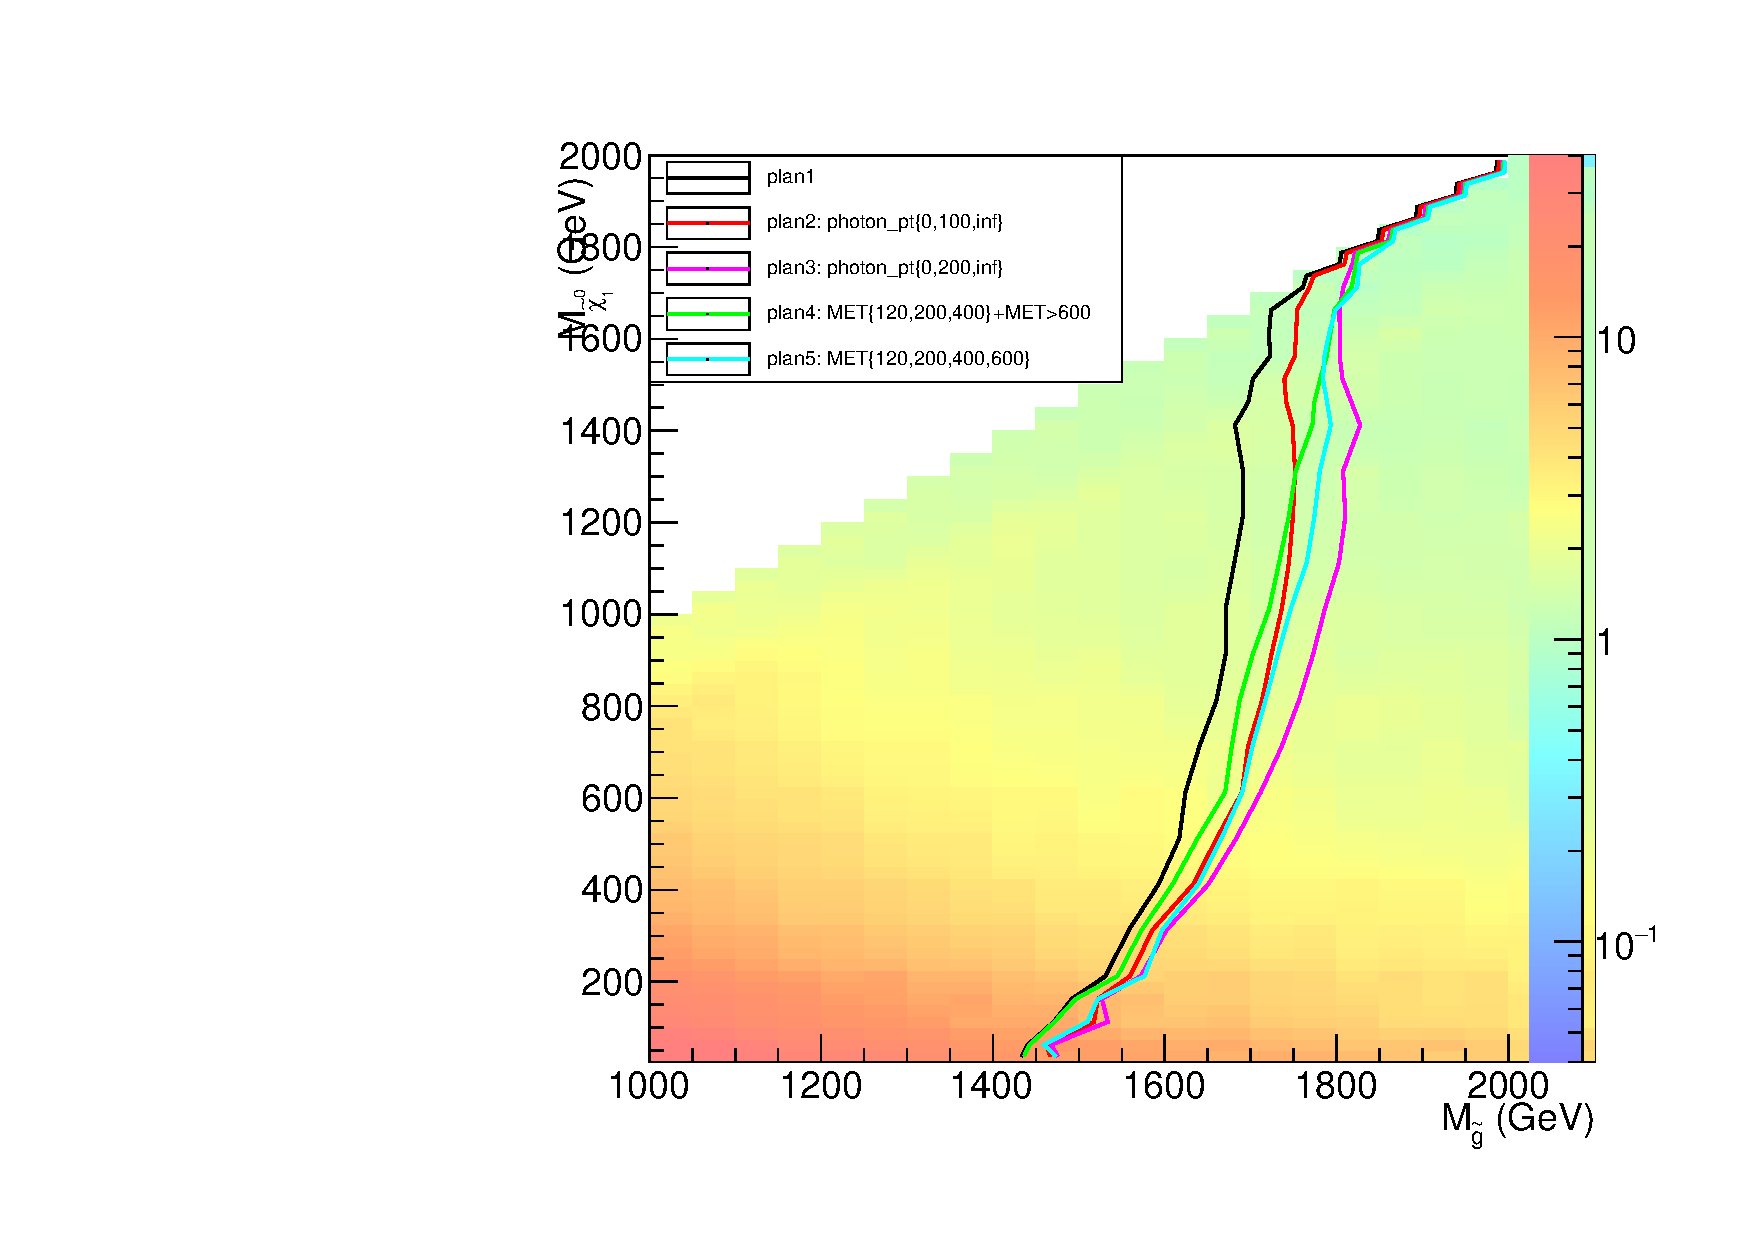
\includegraphics[width=0.49\textwidth]{Figures/binningOpt.pdf}
		\caption{Optimization of the signal bins. Baseline binning (black): $p_T^{miss}$\{120-200, 200-400, $ >$ 400\}GeV $\times$ HT\{ $<$100, 100-400, $ >$ 400\}GeV. Plan 2 (red): $p_T^{miss}$\{120-200, 200-400, $ >$ 400\}GeV $\times$ HT\{ $<$100, 100-400, $ >$ 400\}GeV $\times$ $p_T^\gamma$ \{$<$ 100, $>$ 100\}GeV. Plan 3 (magenta): $p_T^{miss}$\{120-200, 200-400, $ >$ 400\}GeV $\times$ HT\{ $<$100, 100-400, $ >$ 400\}GeV $\times$ $p_T^\gamma$ \{$<$ 200, $>$ 200\}GeV. Plan 4 (green): $p_T^{miss}$\{120-200, 200-400, 400-600\}GeV $\times$ HT\{ $<$100, 100-400, $ >$ 400\}GeV. + \{$p_T^{miss} > $ 600 GeV\}. Plan 5 (cyan): $p_T^{miss}$\{120-200, 200-400, 400-600\}GeV $\times$ HT\{ $<$100, 100-400, $ >$ 400\}GeV. + \{$p_T^{miss} > $ 600 GeV\}$\times$ HT\{ $<$ 400, $ >$ 400\}GeV. }
    \label{fig:signalPhoPt}
\end{figure}

\begin{figure}
  \centering
    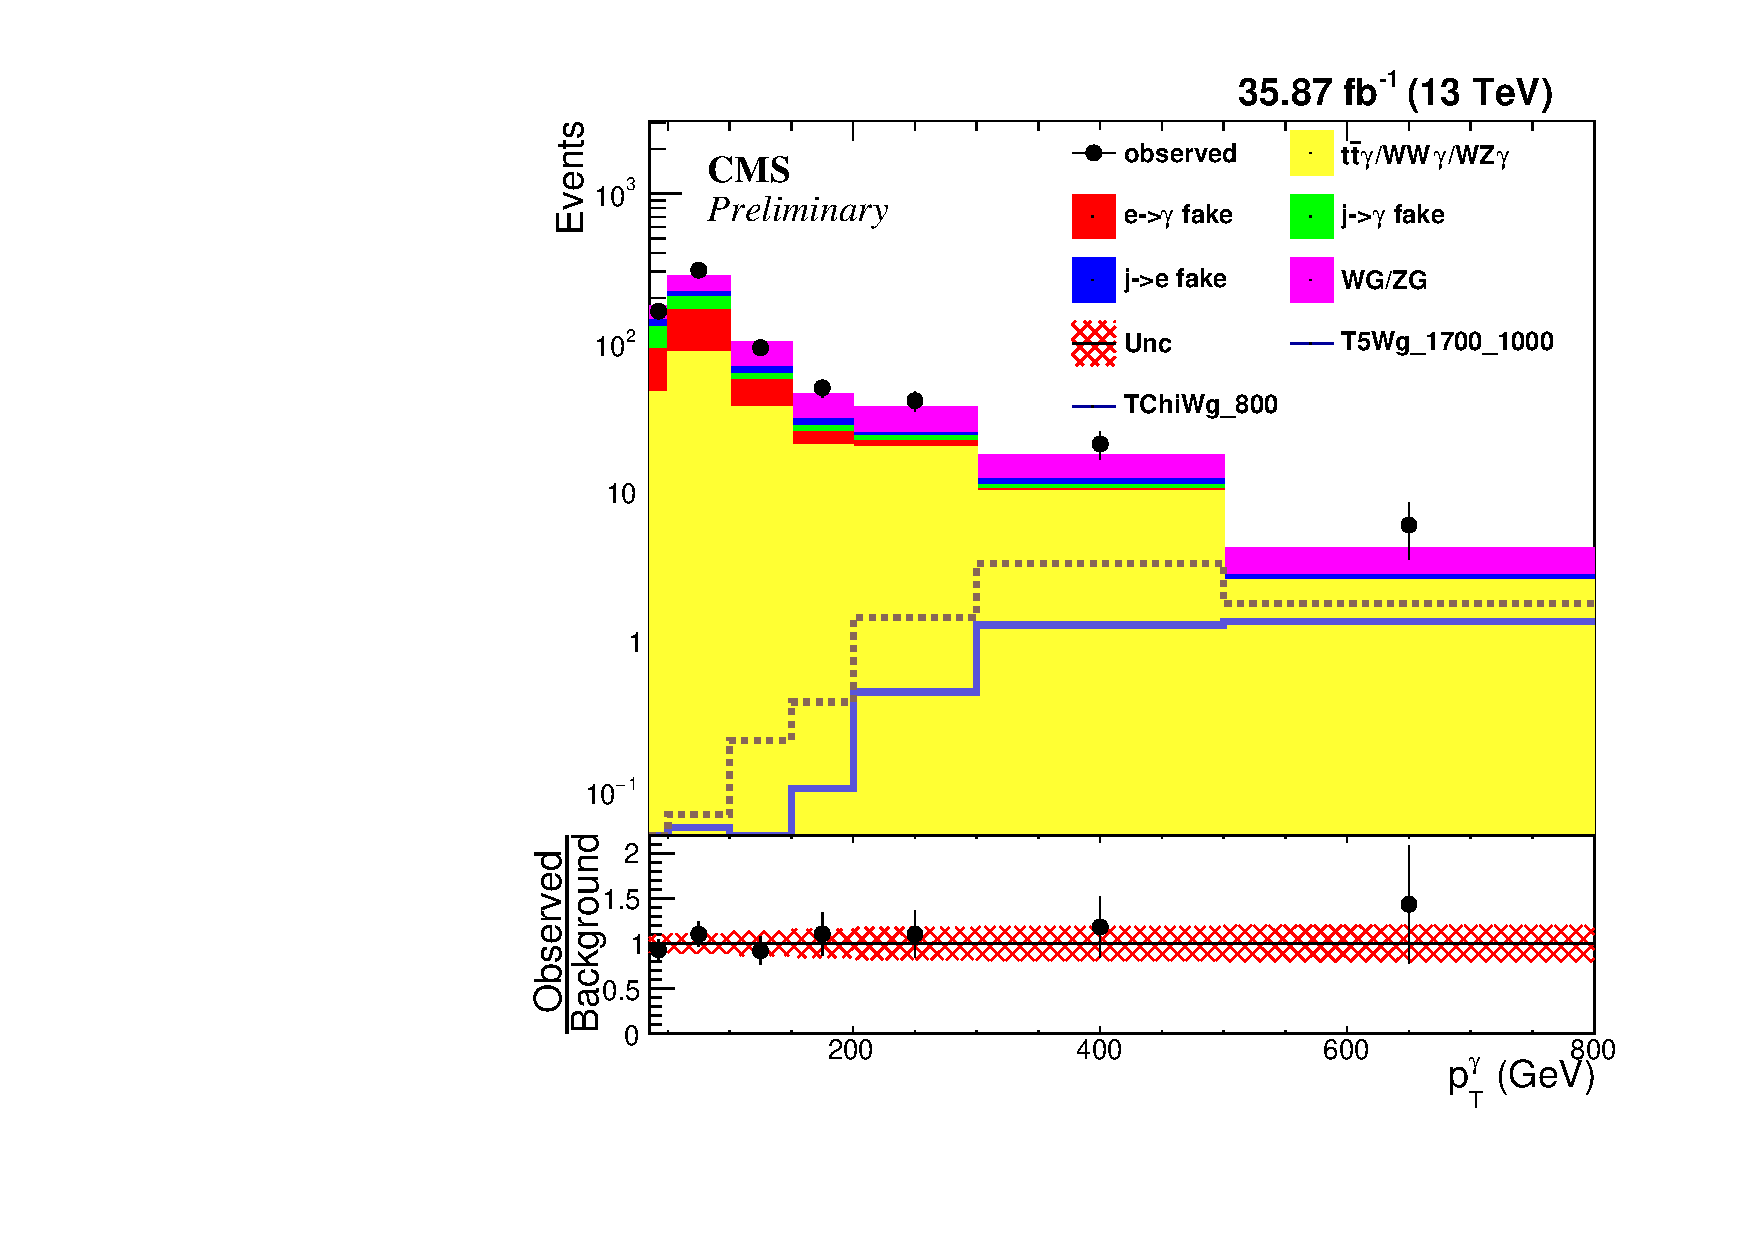
\includegraphics[width=0.49\textwidth]{Figures/SIGNAL_egamma_2016ReMiniAOD_pt.pdf}
		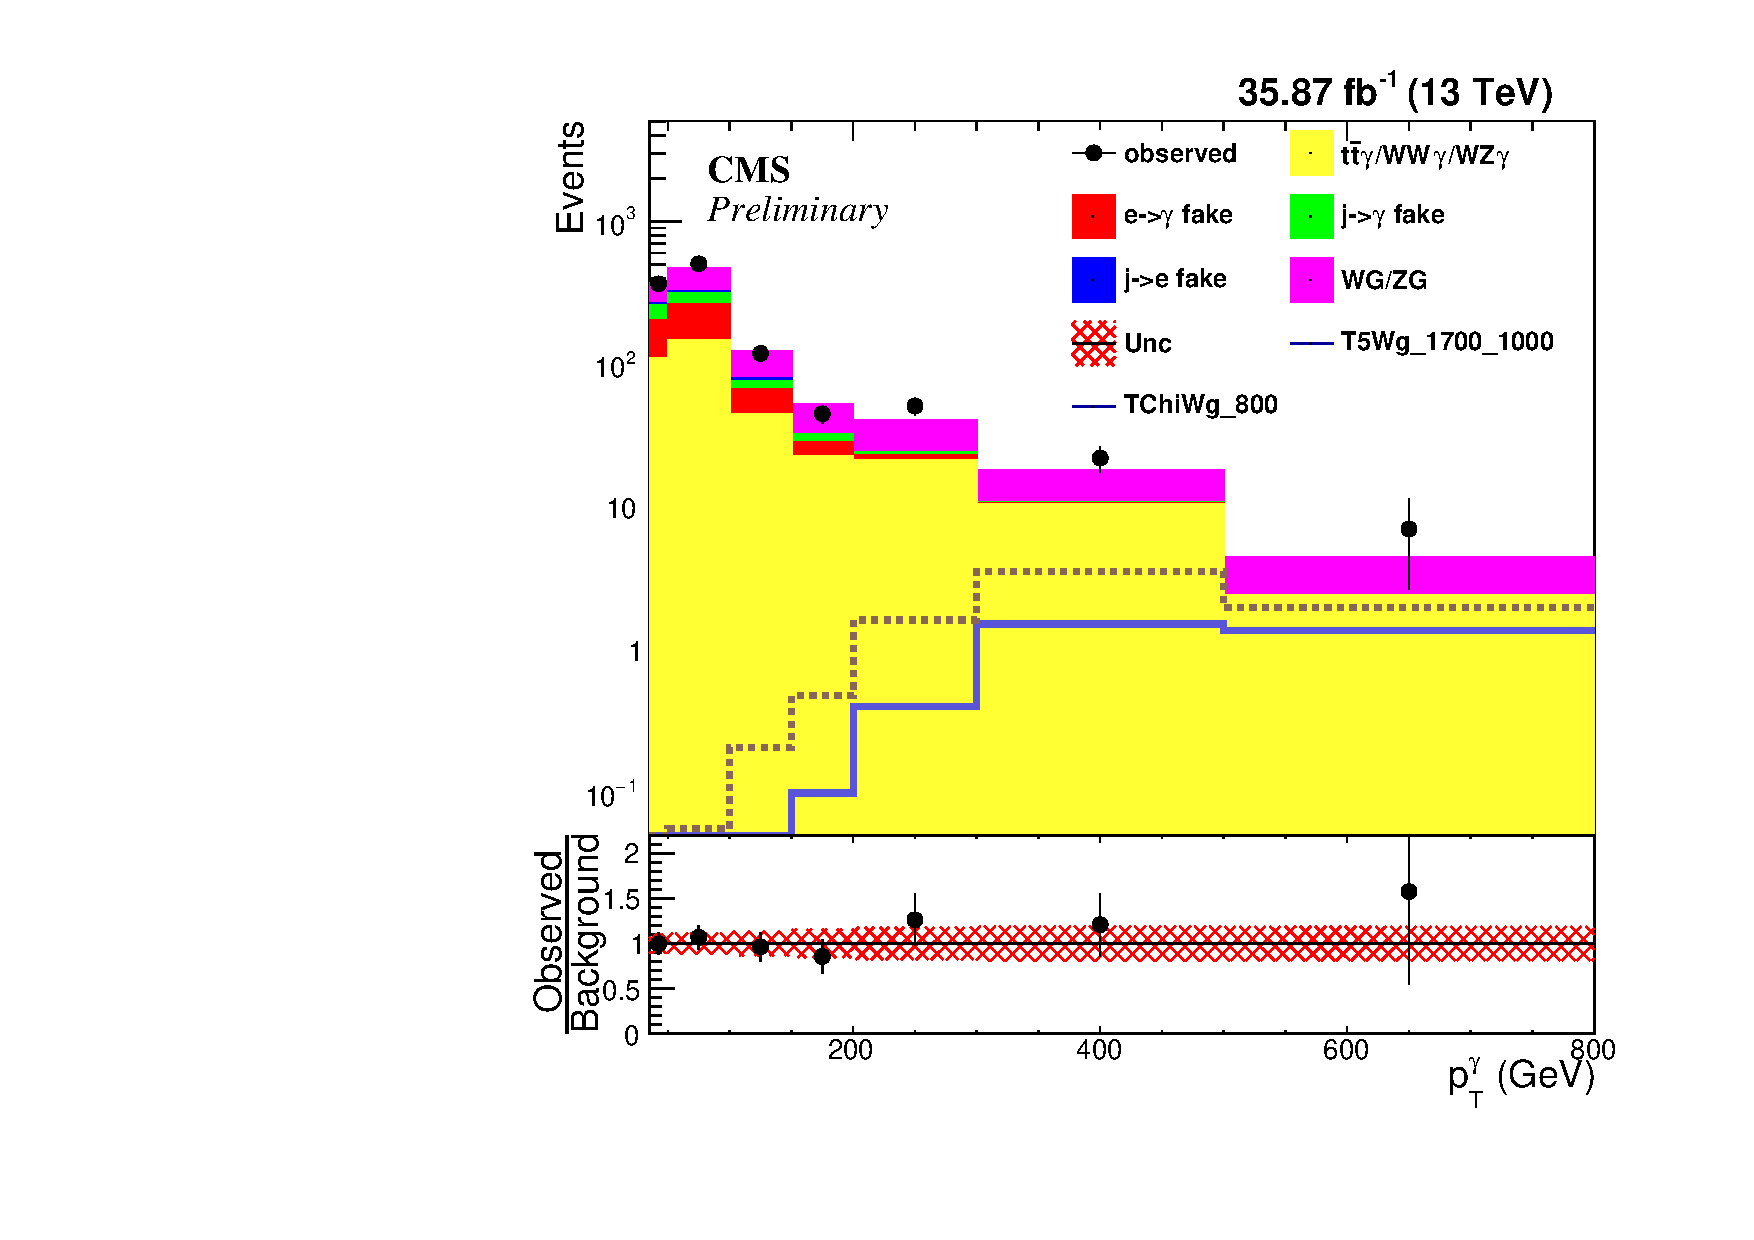
\includegraphics[width=0.49\textwidth]{Figures/SIGNAL_mg_2016ReMiniAOD_pt.pdf}
		\caption{Photon $p_T$ distribution of the observed data and predicted background in the signal region. Left: $e\gamma$, right: $\mu\gamma$}
    \label{fig:signalPhoPt}
\end{figure}

\begin{figure}
  \centering
    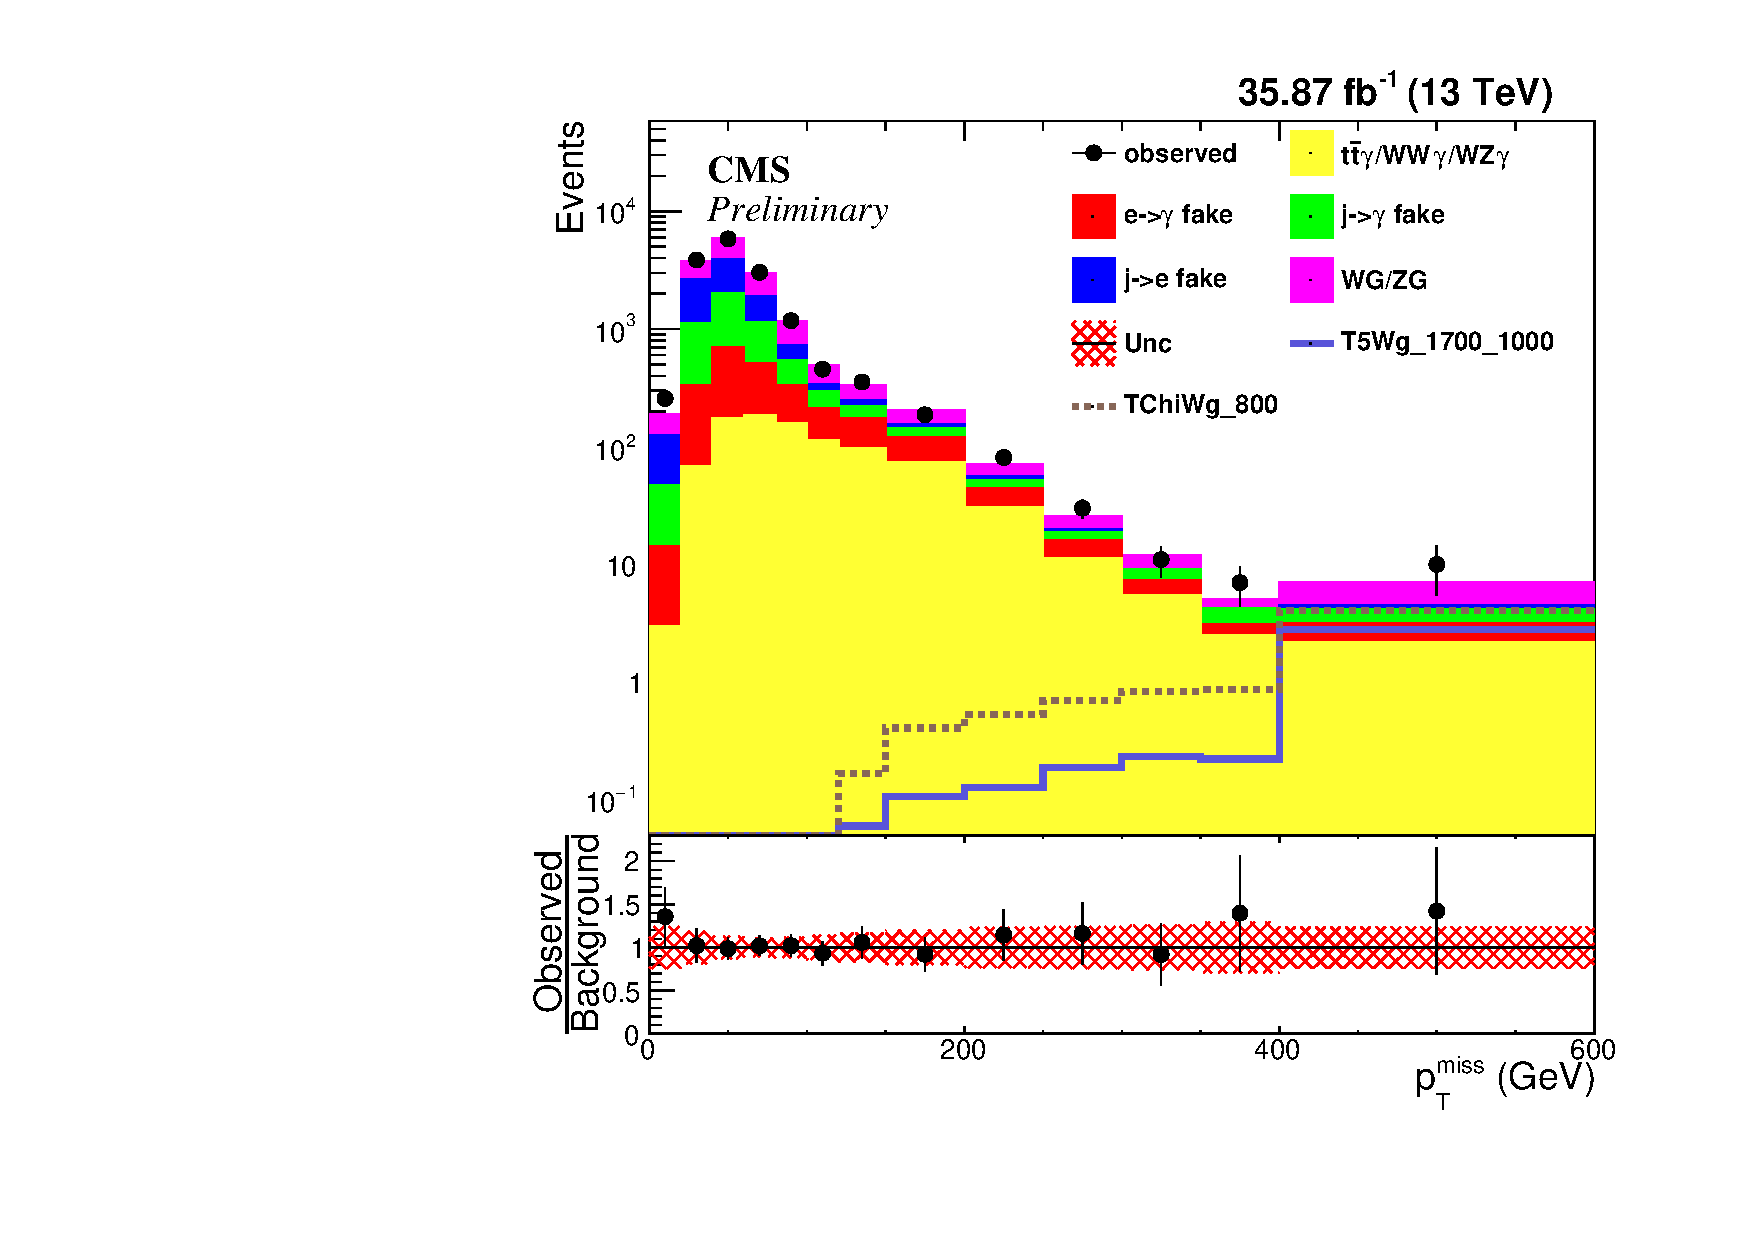
\includegraphics[width=0.49\textwidth]{Figures/SIGNAL_egamma_2016ReMiniAOD_met.pdf}
		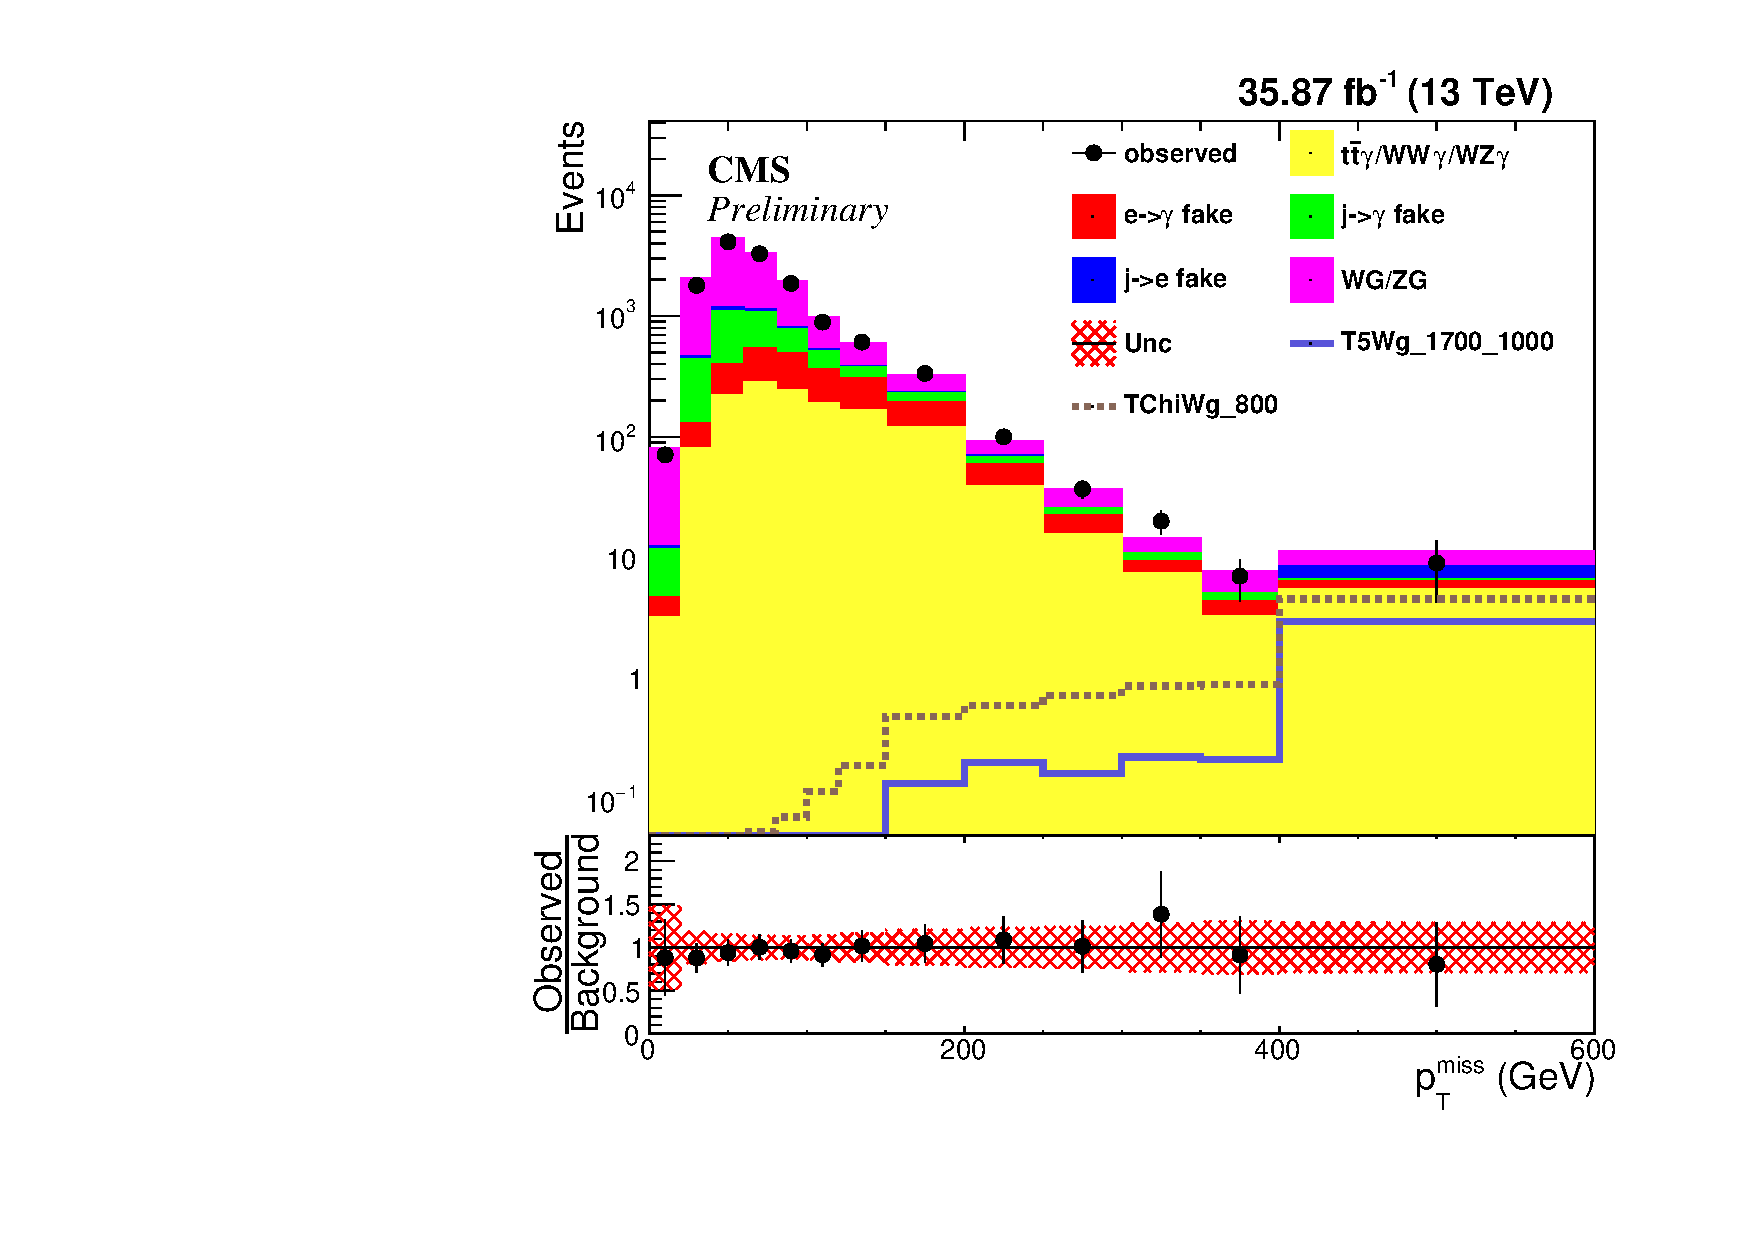
\includegraphics[width=0.49\textwidth]{Figures/SIGNAL_mg_2016ReMiniAOD_met.pdf}
		\caption{$p_T^{miss}$ distribution of the observed data and predicted background in the signal region. Left: $e\gamma$, right: $\mu\gamma$}
    \label{fig:signalMET}
\end{figure}

\begin{figure}
  \centering
    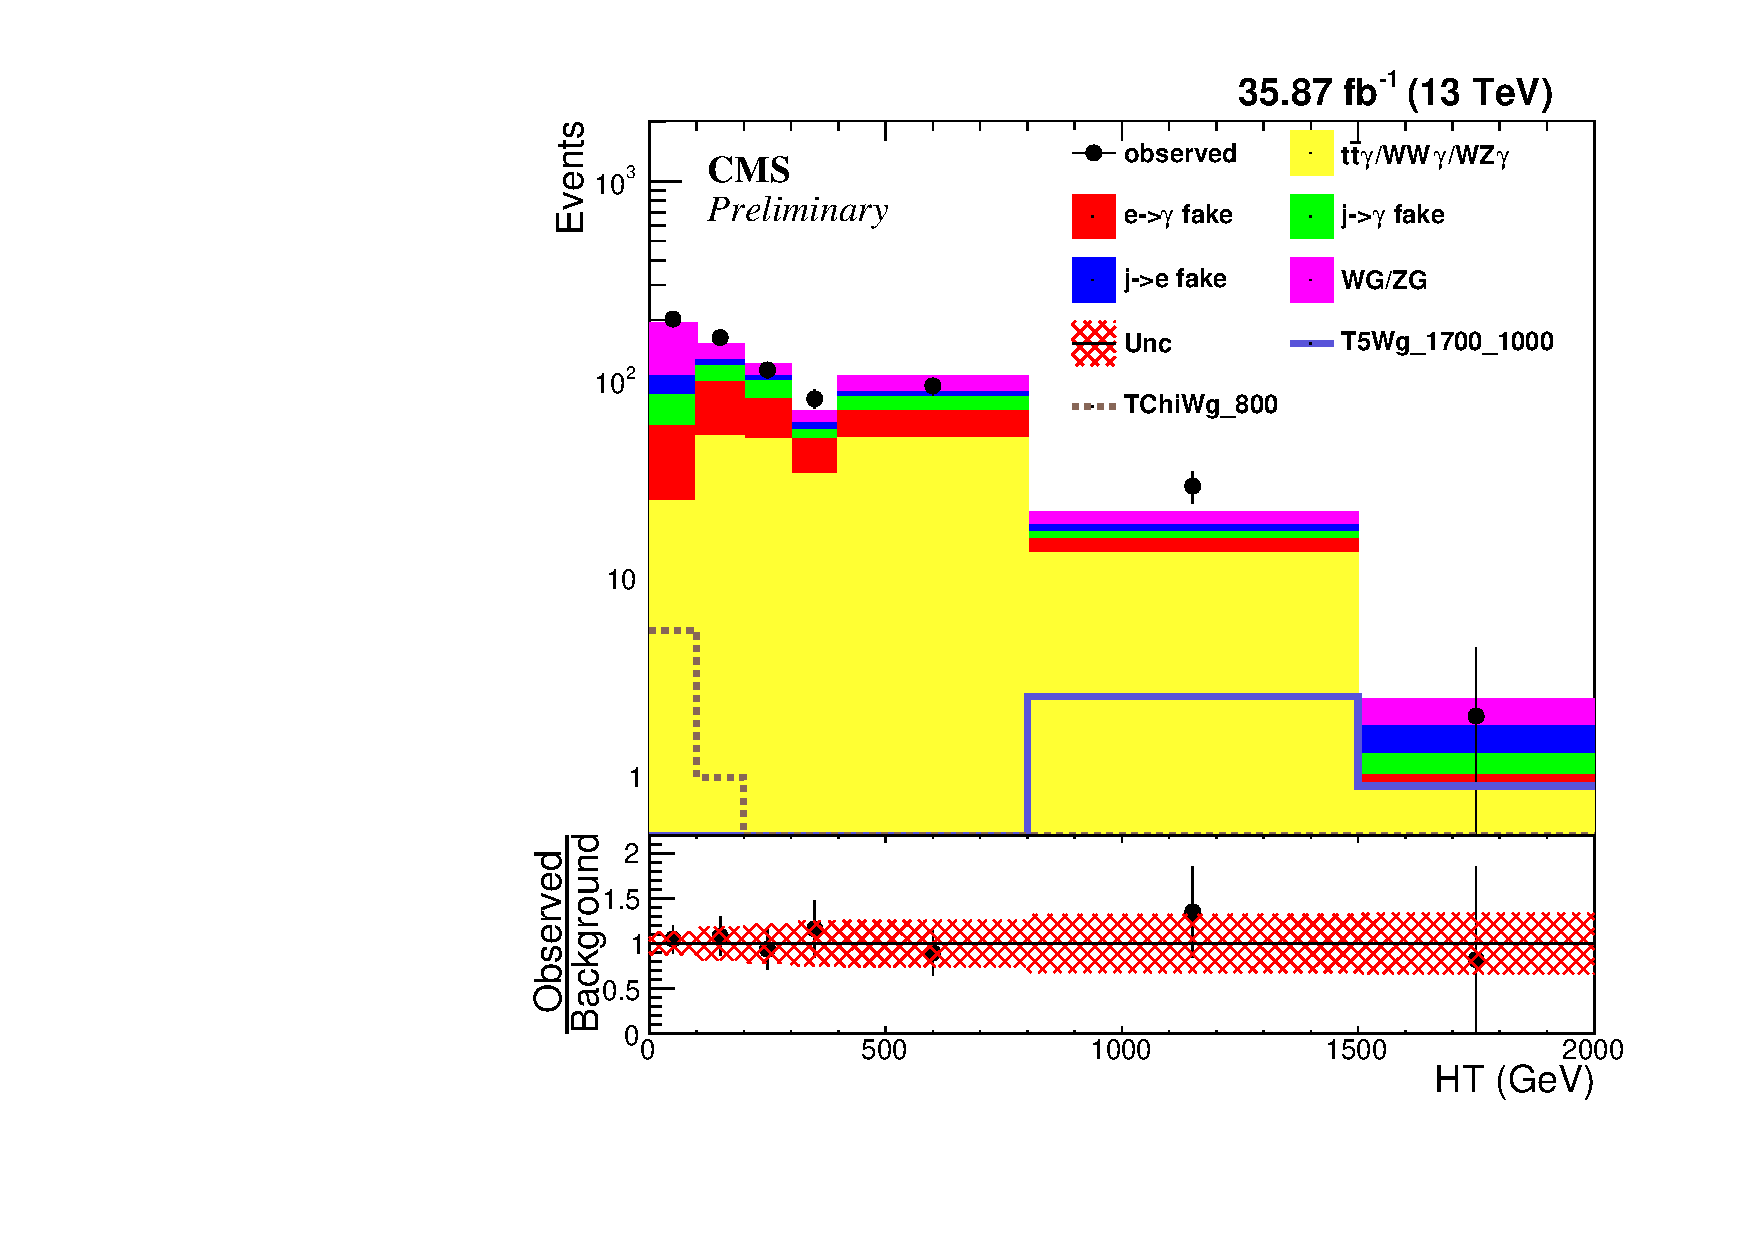
\includegraphics[width=0.49\textwidth]{Figures/SIGNAL_egamma_2016ReMiniAOD_ht.pdf}
		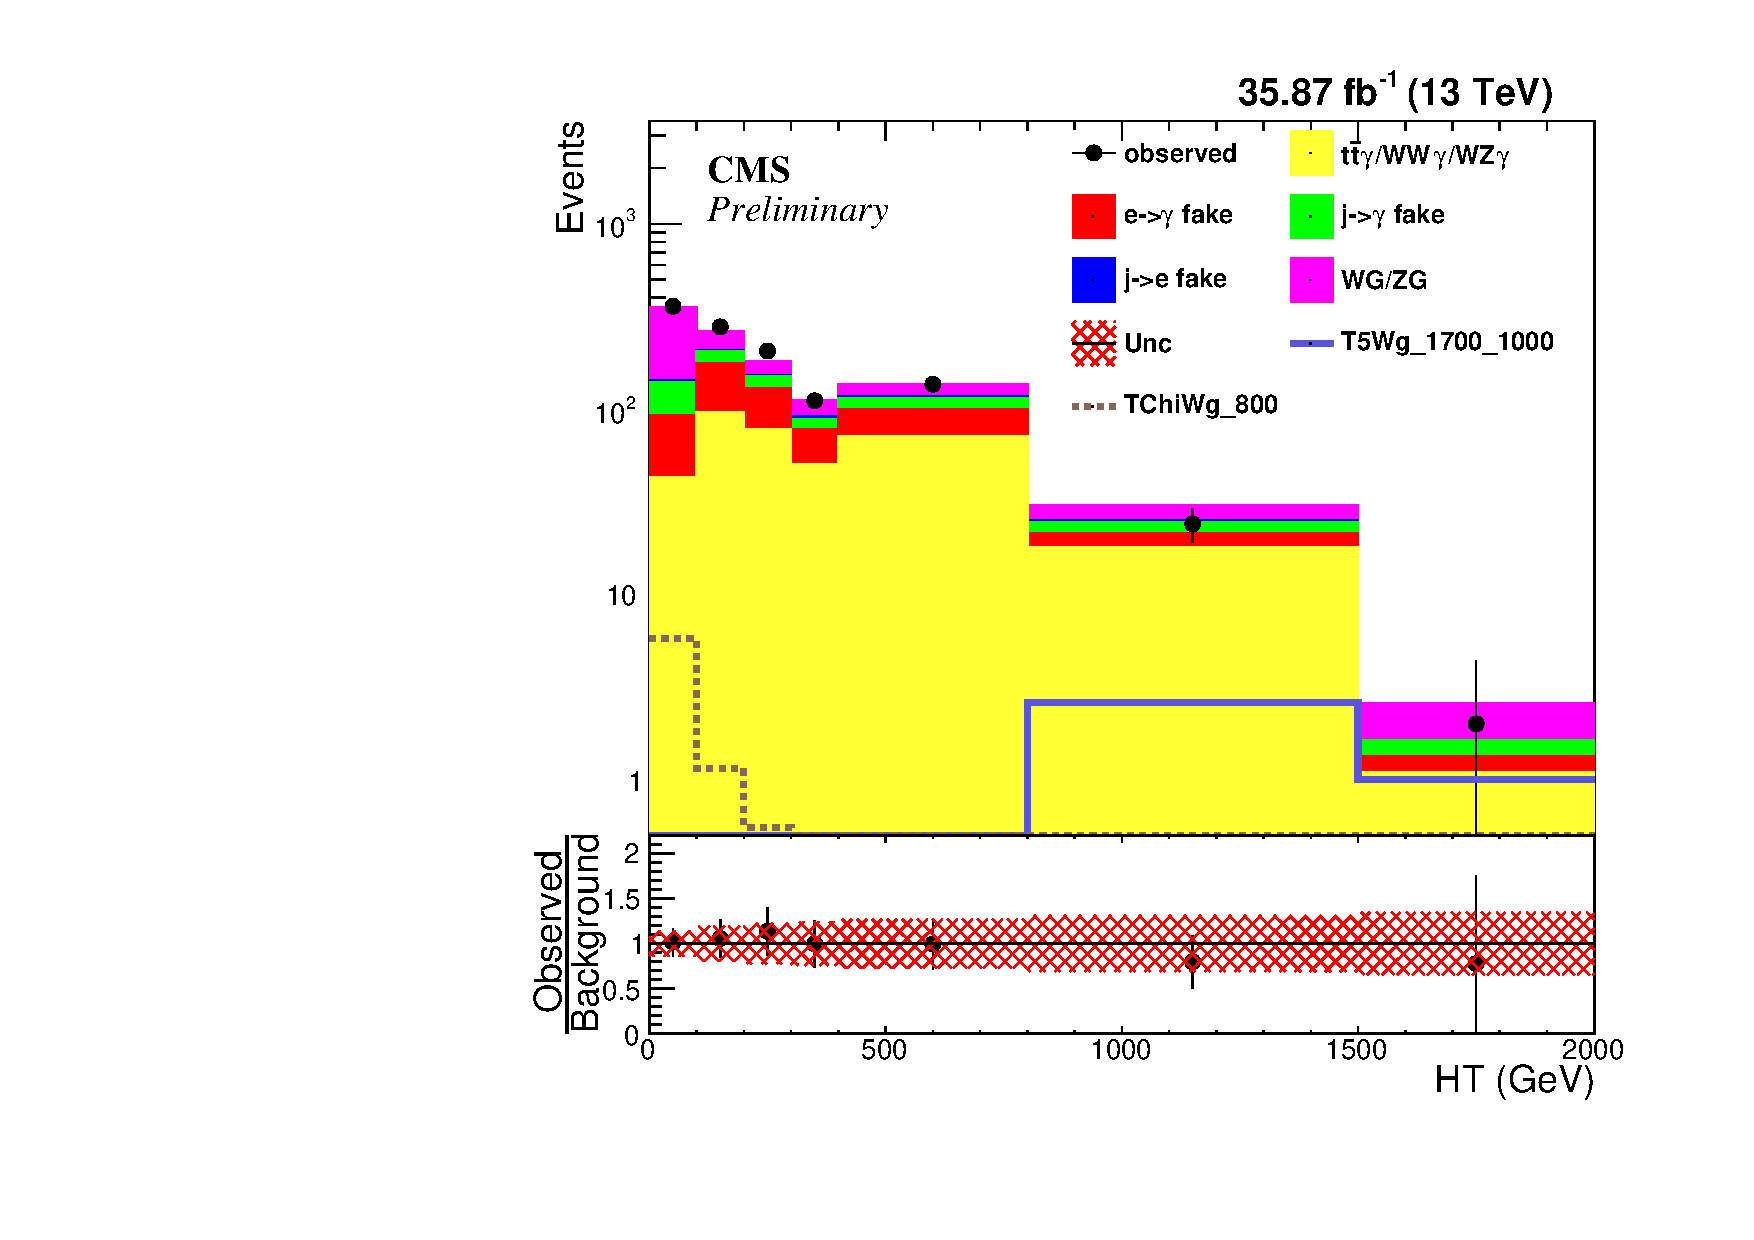
\includegraphics[width=0.49\textwidth]{Figures/SIGNAL_mg_2016ReMiniAOD_ht.pdf}
		\caption{HT distribution of the observed data and predicted background in the signal region. Left: $e\gamma$, right: $\mu\gamma$}
    \label{fig:signalHT}
\end{figure}

\begin{figure}
  \centering
    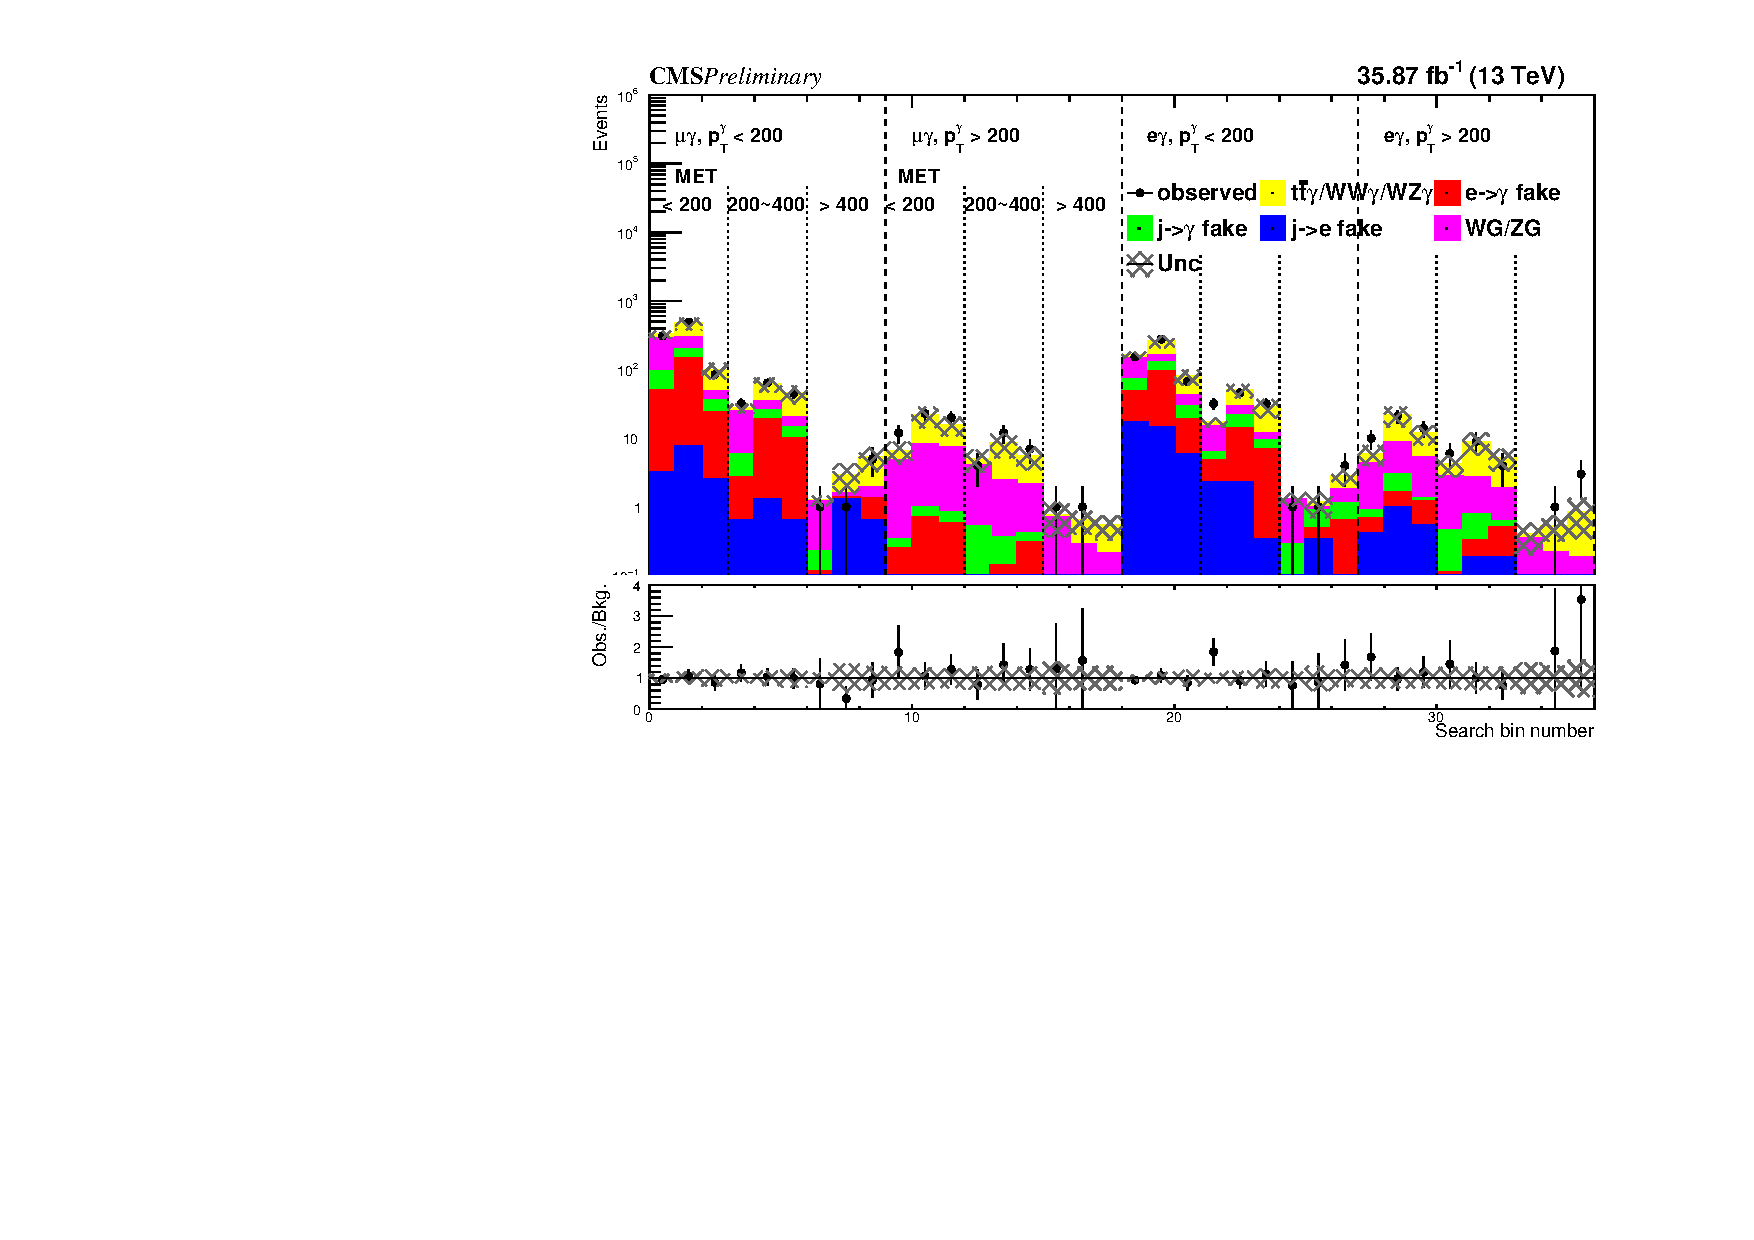
\includegraphics[width=0.9\textwidth]{Figures/signalCount.pdf}
		\caption{Event yields and stacked background predictions as a function of search bin numbers.}
    \label{fig:eventyield}
\end{figure}

\begin{table}[htdp]
 \resizebox{\textwidth}{!}{ 
   \begin{tabular}{|c|c|c|c|c|c|c|c|c|c||c|c|}    
    \hline
	Bin& channel & $p_T^{miss}$ & HT  & $p_T^{\gamma}$ & $e\rightarrow\gamma$ fakes & jet$\rightarrow\gamma$ fakes & jet$\rightarrow l$ fakes  & $W\gamma/Z\gamma$ & rare & SM background & Data \\ \hline 
  1&  $\mu\gamma$   & 120-200 & $<$100  & $<$200  &  46.920 $\pm$ 3.905  &  44.067 $\pm$ 4.611 &   3.100 $\pm$ 1.519  & 183.161 $\pm$ 45.284 &  37.238 $\pm$ 19.051 & 314.486 $\pm$  49.522  & 309\\ \hline
  2&  $\mu\gamma$   & 120-200 & 100-400 & $<$200  & 140.845 $\pm$11.790  &  52.269 $\pm$ 5.214 &   7.440 $\pm$ 2.613  &  85.740 $\pm$ 27.722 & 176.442 $\pm$ 89.401 & 462.736 $\pm$  94.661  & 494\\ \hline
  3&  $\mu\gamma$   & 120-200 & $>$400  & $<$200  & 21.039 $\pm$ 2.085  &  12.701 $\pm$ 1.808 &   2.480 $\pm$ 1.336  &   11.665 $\pm$  4.425 &  50.288 $\pm$ 25.599 &  98.173 $\pm$  26.409  &  85\\ \hline
  4&  $\mu\gamma$   & 200-400 & $<$100  & $<$200  &   2.043 $\pm$ 0.279  &   3.217 $\pm$ 0.780 &   0.620 $\pm$ 0.632  &  17.609 $\pm$  4.476 &   2.837 $\pm$  1.603 &  26.326 $\pm$   4.867  &  32\\ \hline
  5&  $\mu\gamma$   & 200-400 & 100-400 & $<$200  &     17.600 $\pm$ 1.654  &   6.547 $\pm$ 1.193 &   1.240 $\pm$ 0.911  &   8.522 $\pm$  3.794 &  26.959 $\pm$ 13.802 &  60.869 $\pm$  14.502  &  64\\ \hline
  6&  $\mu\gamma$   & 200-400 & $>$400  & $<$200  &     9.351 $\pm$ 1.028  &   4.561 $\pm$ 0.987 &   0.620 $\pm$ 0.632  &   5.246 $\pm$  2.922 &  25.095 $\pm$ 12.899 &  44.873 $\pm$  13.325  &  45\\ \hline
  7&  $\mu\gamma$   & $>$400 & $<$100   & $<$200  &     0.116 $\pm$ 0.055  &   0.108 $\pm$ 0.113 &   0.000 $\pm$ 0.000  &   0.931 $\pm$  0.217 &   0.031 $\pm$  0.023 &   1.187 $\pm$   0.252  &   1\\ \hline
  8&  $\mu\gamma$   & $>$400 & 100-400  & $<$200  &     0.108 $\pm$ 0.043  &   0.000 $\pm$ 0.000 &   1.240 $\pm$ 0.912  &   0.169 $\pm$  0.100 &   1.352 $\pm$  0.997 &   2.869 $\pm$   1.355  &   1\\ \hline
  9&  $\mu\gamma$   & $>$400 & $>$400   & $<$200  &     0.686 $\pm$ 0.133  &   0.000 $\pm$ 0.000 &   0.620 $\pm$ 0.632  &   0.598 $\pm$  0.350 &   3.358 $\pm$  1.897 &   5.262 $\pm$   2.034  &   5\\ \hline
 10&  $\mu\gamma$   & 120-200 & $<$100  & $>$200  &     0.248 $\pm$ 0.096  &   0.096 $\pm$ 0.090 &   0.000 $\pm$ 0.000  &   4.294 $\pm$  2.207 &   1.673 $\pm$  0.868 &   6.312 $\pm$   2.374  &  12\\ \hline
 11&  $\mu\gamma$   & 120-200 & 100-400 & $>$200  &     0.715 $\pm$ 0.243  &   0.270 $\pm$ 0.192 &   0.000 $\pm$ 0.000  &   6.938 $\pm$  2.776 &  13.164 $\pm$  6.688 &  21.086 $\pm$   7.219  &  23\\ \hline
 12&  $\mu\gamma$   & 120-200 & $>$400  & $>$200  &     0.580 $\pm$ 0.209  &   0.265 $\pm$ 0.182 &   0.000 $\pm$ 0.000  &   6.255 $\pm$  2.378 &   8.149 $\pm$  4.251 &  15.248 $\pm$   4.885  &  20\\ \hline
 13&  $\mu\gamma$   & 200-400 & $<$100  & $>$200  &     0.081 $\pm$ 0.037  &   0.438 $\pm$ 0.258 &   0.000 $\pm$ 0.000  &   3.398 $\pm$  1.736 &   0.916 $\pm$  0.473 &   4.833 $\pm$   1.818  &   4\\ \hline
 14&  $\mu\gamma$   & 200-400 & 100-400 & $>$200  &     0.142 $\pm$ 0.061  &   0.223 $\pm$ 0.161 &   0.000 $\pm$ 0.000  &   1.948 $\pm$  1.004 &   5.952 $\pm$  3.017 &   8.265 $\pm$   3.185  &  12\\ \hline
 15&  $\mu\gamma$   & 200-400 & $>$400  & $>$200  &     0.302 $\pm$ 0.115  &   0.118 $\pm$ 0.103 &   0.000 $\pm$ 0.000  &   1.607 $\pm$  0.889 &   3.347 $\pm$  1.736 &   5.374 $\pm$   1.957  &   7\\ \hline
 16&  $\mu\gamma$   & $>$400 & $<$100   & $>$200  &     0.000 $\pm$ 0.000  &   0.000 $\pm$ 0.000 &   0.000 $\pm$ 0.000  &   0.679 $\pm$  0.398 &   0.051 $\pm$  0.036 &   0.730 $\pm$   0.397  &   1\\ \hline
 17&  $\mu\gamma$   & $>$400 & 100-400  & $>$200  &     0.010 $\pm$ 0.008  &   0.057 $\pm$ 0.064 &   0.000 $\pm$ 0.000  &   0.208 $\pm$  0.126 &   0.348 $\pm$  0.185 &   0.623 $\pm$   0.234  &   1\\ \hline
 18&  $\mu\gamma$   & $>$400 & $>$400   & $>$200  &     0.025 $\pm$ 0.015  &   0.000 $\pm$ 0.000 &   0.000 $\pm$ 0.000  &   0.178 $\pm$  0.113 &   0.326 $\pm$  0.174 &   0.529 $\pm$   0.209  &   0\\ \hline
 \hline
 19&  $e\gamma$     & 120-200 & $<$100  & $<$200  &    30.691 $\pm$ 2.748  &  23.562 $\pm$ 2.985 &  17.260 $\pm$ 4.153  &  72.967 $\pm$ 10.793 &  19.145 $\pm$  9.884 & 163.626 $\pm$  15.745  & 153\\ \hline
 20&  $e\gamma$     & 120-200 & 100-400 & $<$200  &   79.791 $\pm$ 7.376  &  33.203 $\pm$ 3.721 &  14.430 $\pm$ 4.280  &  35.227 $\pm$ 12.349 &  94.304 $\pm$ 47.654 & 256.955 $\pm$  50.100  & 277\\ \hline
 21&  $e\gamma$     & 120-200 & $>$400  & $<$200  &    13.083 $\pm$ 1.442  &  10.713 $\pm$ 1.785 &   5.778 $\pm$ 1.880  &  12.160 $\pm$  5.883 &  37.216 $\pm$ 18.867 &  78.950 $\pm$  19.984  &  67\\ \hline
 22&  $e\gamma$     & 200-400 & $<$100  & $<$200  &     2.485 $\pm$ 0.326  &   1.478 $\pm$ 0.590 &   2.314 $\pm$ 1.340  &   8.903 $\pm$  1.876 &   2.129 $\pm$  1.154 &  17.309 $\pm$   2.664  &  32\\ \hline
 23&  $e\gamma$     & 200-400 & 100-400 & $<$200  &    11.659 $\pm$ 1.149  &   8.026 $\pm$ 1.514 &   2.298 $\pm$ 1.023  &   7.126 $\pm$  2.859 &  20.846 $\pm$ 10.636 &  49.956 $\pm$  11.223  &  46\\ \hline
 24&  $e\gamma$     & 200-400 & $>$400  & $<$200  &     6.479 $\pm$ 0.787  &   2.465 $\pm$ 0.772 &   0.336 $\pm$ 0.365  &   2.511 $\pm$  1.375 &  16.372 $\pm$  8.417 &  28.164 $\pm$   8.607  &  32\\ \hline
 25&  $e\gamma$     & $>$400 & $<$100   & $<$200  &     0.097 $\pm$ 0.043  &   0.184 $\pm$ 0.185 &   0.000 $\pm$ 0.000  &   0.997 $\pm$  0.190 &   0.023 $\pm$  0.018 &   1.302 $\pm$   0.269  &   1\\ \hline
 26&  $e\gamma$     & $>$400 & 100-400  & $<$200  &     0.160 $\pm$ 0.067  &   0.389 $\pm$ 0.279 &   0.336 $\pm$ 0.352  &   0.111 $\pm$  0.053 &   0.165 $\pm$  0.091 &   1.160 $\pm$   0.466  &   1\\ \hline
 27&  $e\gamma$     & $>$400 & $>$400   & $<$200  &     0.635 $\pm$ 0.132  &   0.490 $\pm$ 0.308 &   0.000 $\pm$ 0.000  &   0.682 $\pm$  0.410 &   0.997 $\pm$  0.545 &   2.804 $\pm$   0.759  &   4\\ \hline
 28&  $e\gamma$     & 120-200 & $<$100  & $>$200  &     0.262 $\pm$ 0.100  &   0.232 $\pm$ 0.184 &   0.412 $\pm$ 0.450  &   3.376 $\pm$  1.581 &   1.645 $\pm$  1.001 &   5.927 $\pm$   1.936  &  10\\ \hline
 29&  $e\gamma$     & 120-200 & 100-400 & $>$200  &     0.644 $\pm$ 0.221  &   1.393 $\pm$ 0.750 &   0.977 $\pm$ 0.557  &   5.808 $\pm$  2.266 &  12.792 $\pm$  6.472 &  21.614 $\pm$   6.924  &  21\\ \hline
 30&  $e\gamma$     & 120-200 & $>$400  & $>$200  &     0.678 $\pm$ 0.239  &   0.116 $\pm$ 0.132 &   0.535 $\pm$ 0.422  &   3.979 $\pm$  1.501 &   6.368 $\pm$  3.286 &  11.677 $\pm$   3.647  &  14\\ \hline
 31&  $e\gamma$     & 200-400 & $<$100  & $>$200  &     0.113 $\pm$ 0.057  &   0.347 $\pm$ 0.243 &   0.000 $\pm$ 0.000  &   2.320 $\pm$  1.142 &   1.355 $\pm$  0.808 &   4.135 $\pm$   1.421  &   6\\ \hline
 32&  $e\gamma$     & 200-400 & 100-400 & $>$200  &     0.140 $\pm$ 0.056  &   0.467 $\pm$ 0.317 &   0.187 $\pm$ 0.195  &   1.953 $\pm$  0.764 &   6.129 $\pm$  3.115 &   8.876 $\pm$   3.230  &   9\\ \hline
 33&  $e\gamma$     & 200-400 & $>$400  & $>$200  &     0.317 $\pm$ 0.120  &   0.116 $\pm$ 0.131 &   0.187 $\pm$ 0.195  &   1.237 $\pm$  0.632 &   3.266 $\pm$  1.659 &   5.123 $\pm$   1.795  &   4\\ \hline
 34&  $e\gamma$     & $>$400 & $<$100   & $>$200  &     0.009 $\pm$ 0.008  &   0.000 $\pm$ 0.000 &   0.000 $\pm$ 0.000  &   0.341 $\pm$  0.191 &   0.044 $\pm$  0.031 &   0.394 $\pm$   0.194  &   0\\ \hline
 35&  $e\gamma$     & $>$400 & 100-400  & $>$200  &     0.000 $\pm$ 0.000  &   0.000 $\pm$ 0.000 &   0.000 $\pm$ 0.000  &   0.219 $\pm$  0.131 &   0.312 $\pm$  0.169 &   0.532 $\pm$   0.213  &   1\\ \hline
 36&  $e\gamma$     & $>$400 & $>$400   & $>$200  &     0.030 $\pm$ 0.018  &   0.000 $\pm$ 0.000 &   0.000 $\pm$ 0.000  &   0.157 $\pm$  0.096 &   0.660 $\pm$  0.493 &   0.848 $\pm$   0.502  &   3\\ \hline
 \end{tabular}
 }
 \caption{Observed number of events and predicted SM backgrounds in search bins. The systematic uncertainties of each background components are added in quadrature.}
 \label{tab:unblindeddata}
 \end{table}    
}


The results are interpreted in terms of upper limits on the cross sections of three different simplified models: TChiWg, T5Wg and T6Wg, which are described in Section \ref{sec:introduction}. The 95\% confidence level (CL) upper limits are obtained using a asymptotic profiled likelihood as test statistics. The limits for the TChiWg models are shown as function of the NLSP masses in Figure \ref{fig:tchiwglimit}, together with the theoretical cross sections of the $\PSGczDo$/$\PSGcpmDo$ pair production. The search excludes NLSP masses up to 900 GeV. Figure \ref{fig:t5wglimit} shows the upper limits on the cross section $\times$ 50\% BR for the T5Wg (left) and T6Wg (right) events with a chargino and a neutralino. The gluino (squark) mass is excluded up to 1700 (1400) GeV in the T5Wg (T6Wg) scenarios.

\begin{figure}
  \centering
    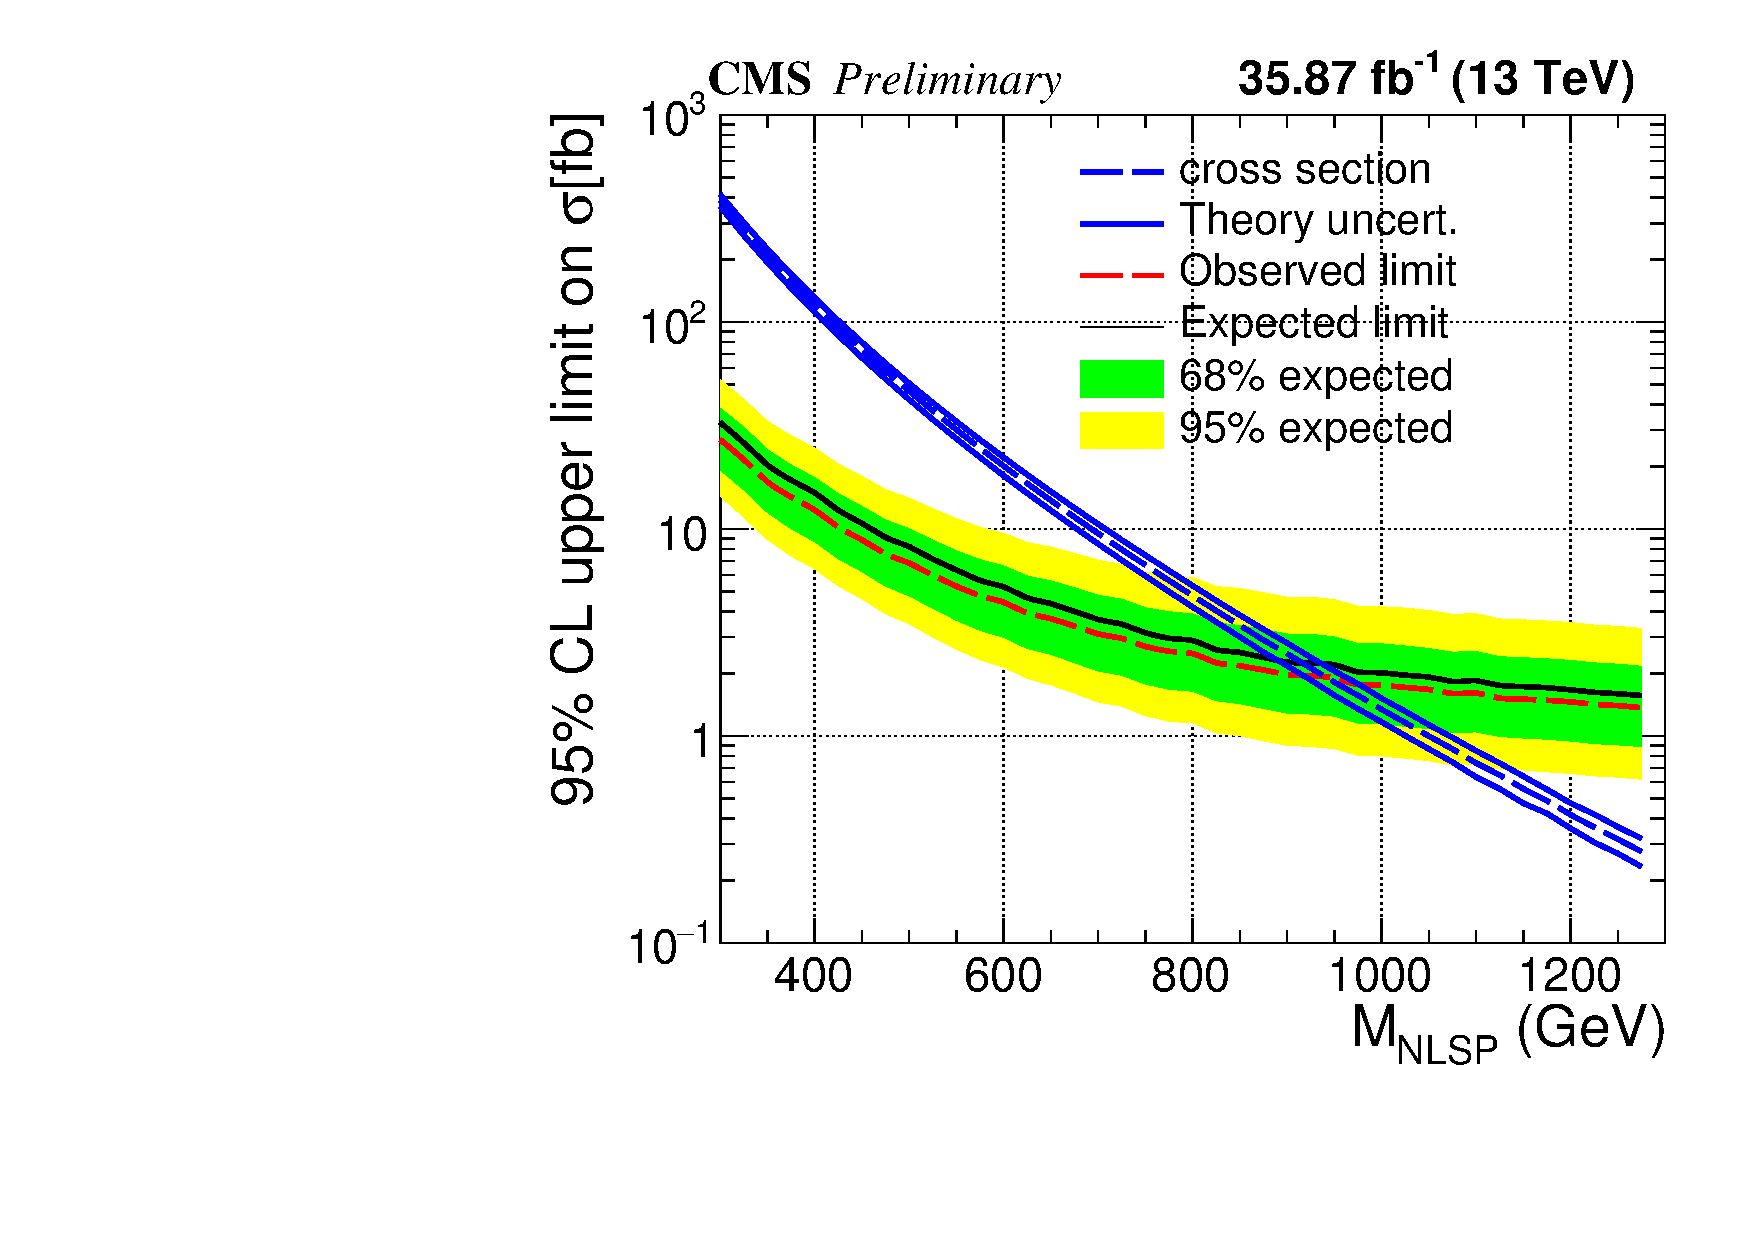
\includegraphics[width=0.7\textwidth]{Figures/TChiWG_limit_Unblind.pdf} 
		\caption{Observed and expected upper limits on the cross sections of the TChiWg model, together with the theoretical cross sections. }
    \label{fig:tchiwglimit}
\end{figure}

\begin{figure}
  \centering
    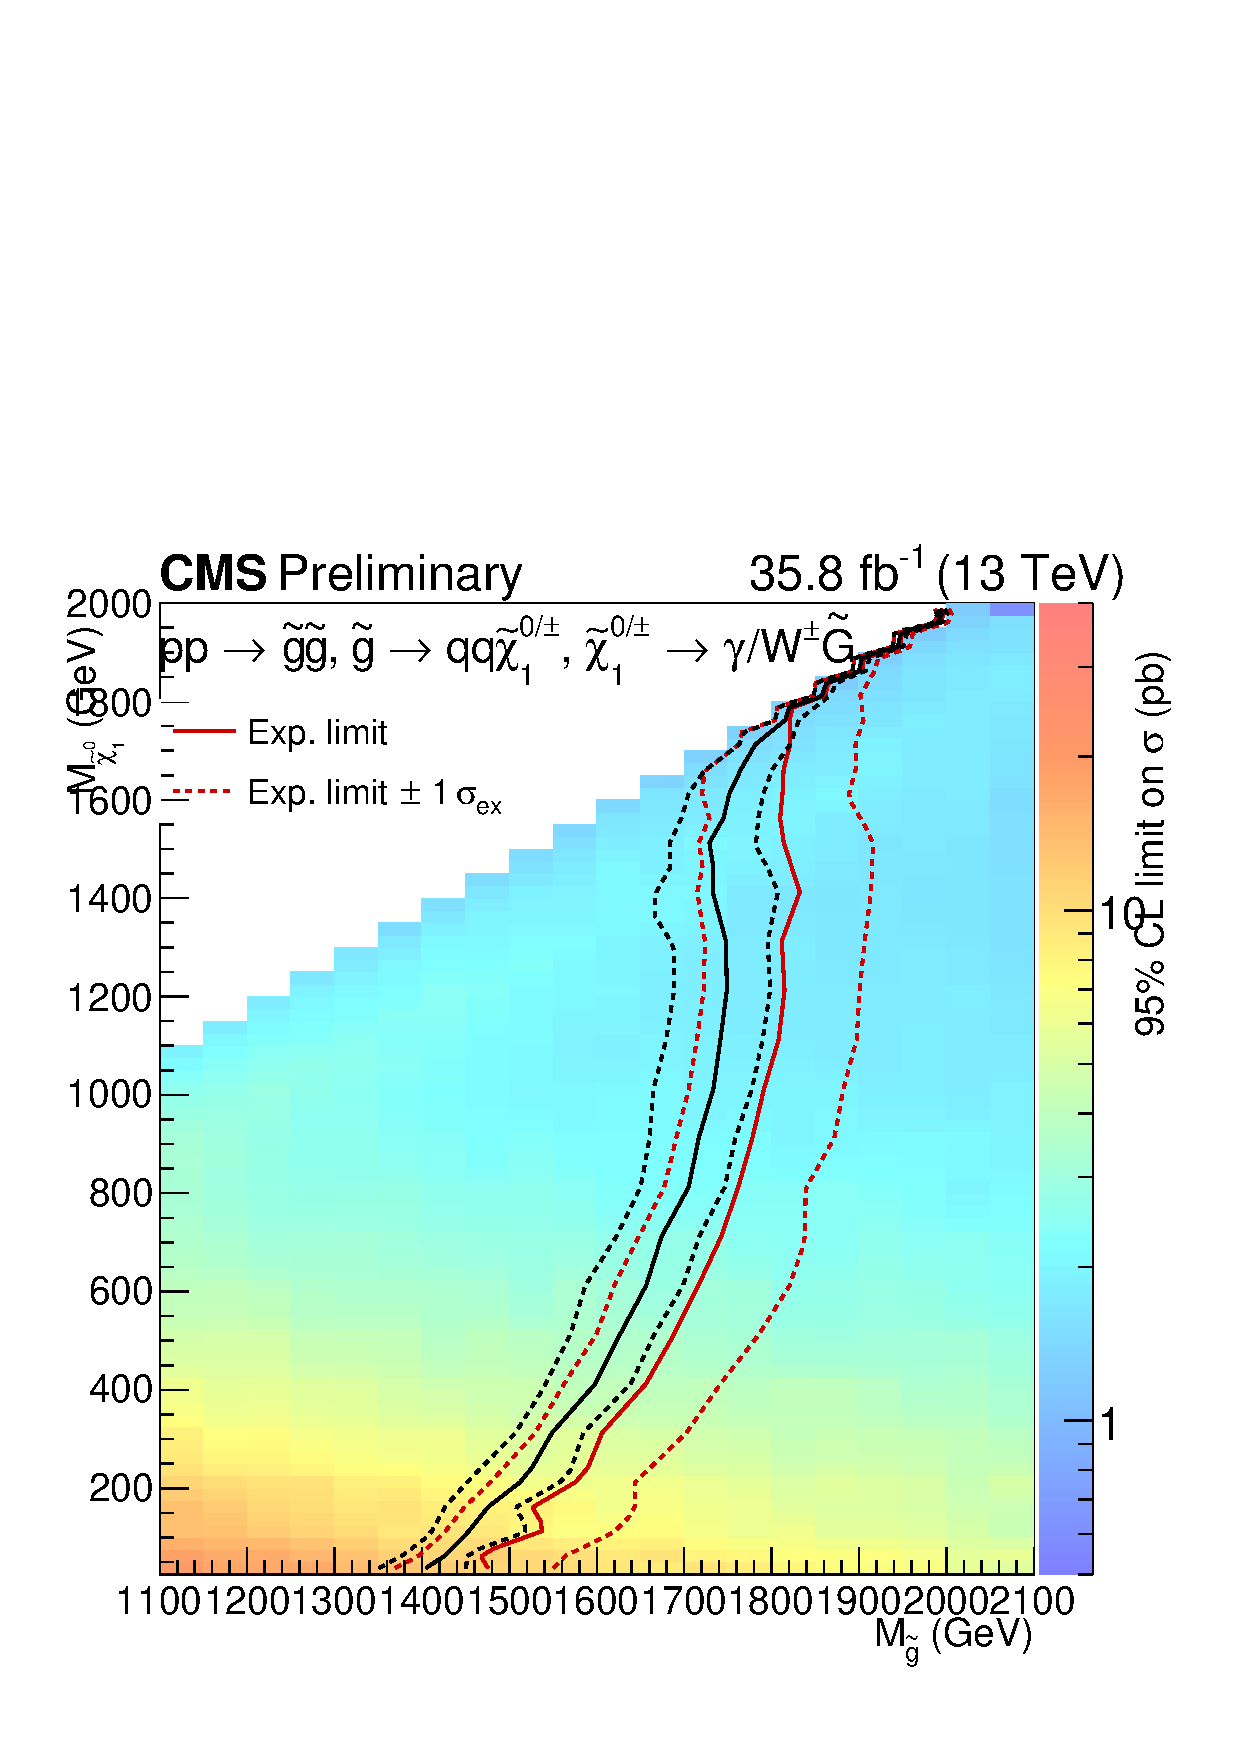
\includegraphics[width=0.49\textwidth]{Figures/T5WG_UnblindLimit.pdf} 
    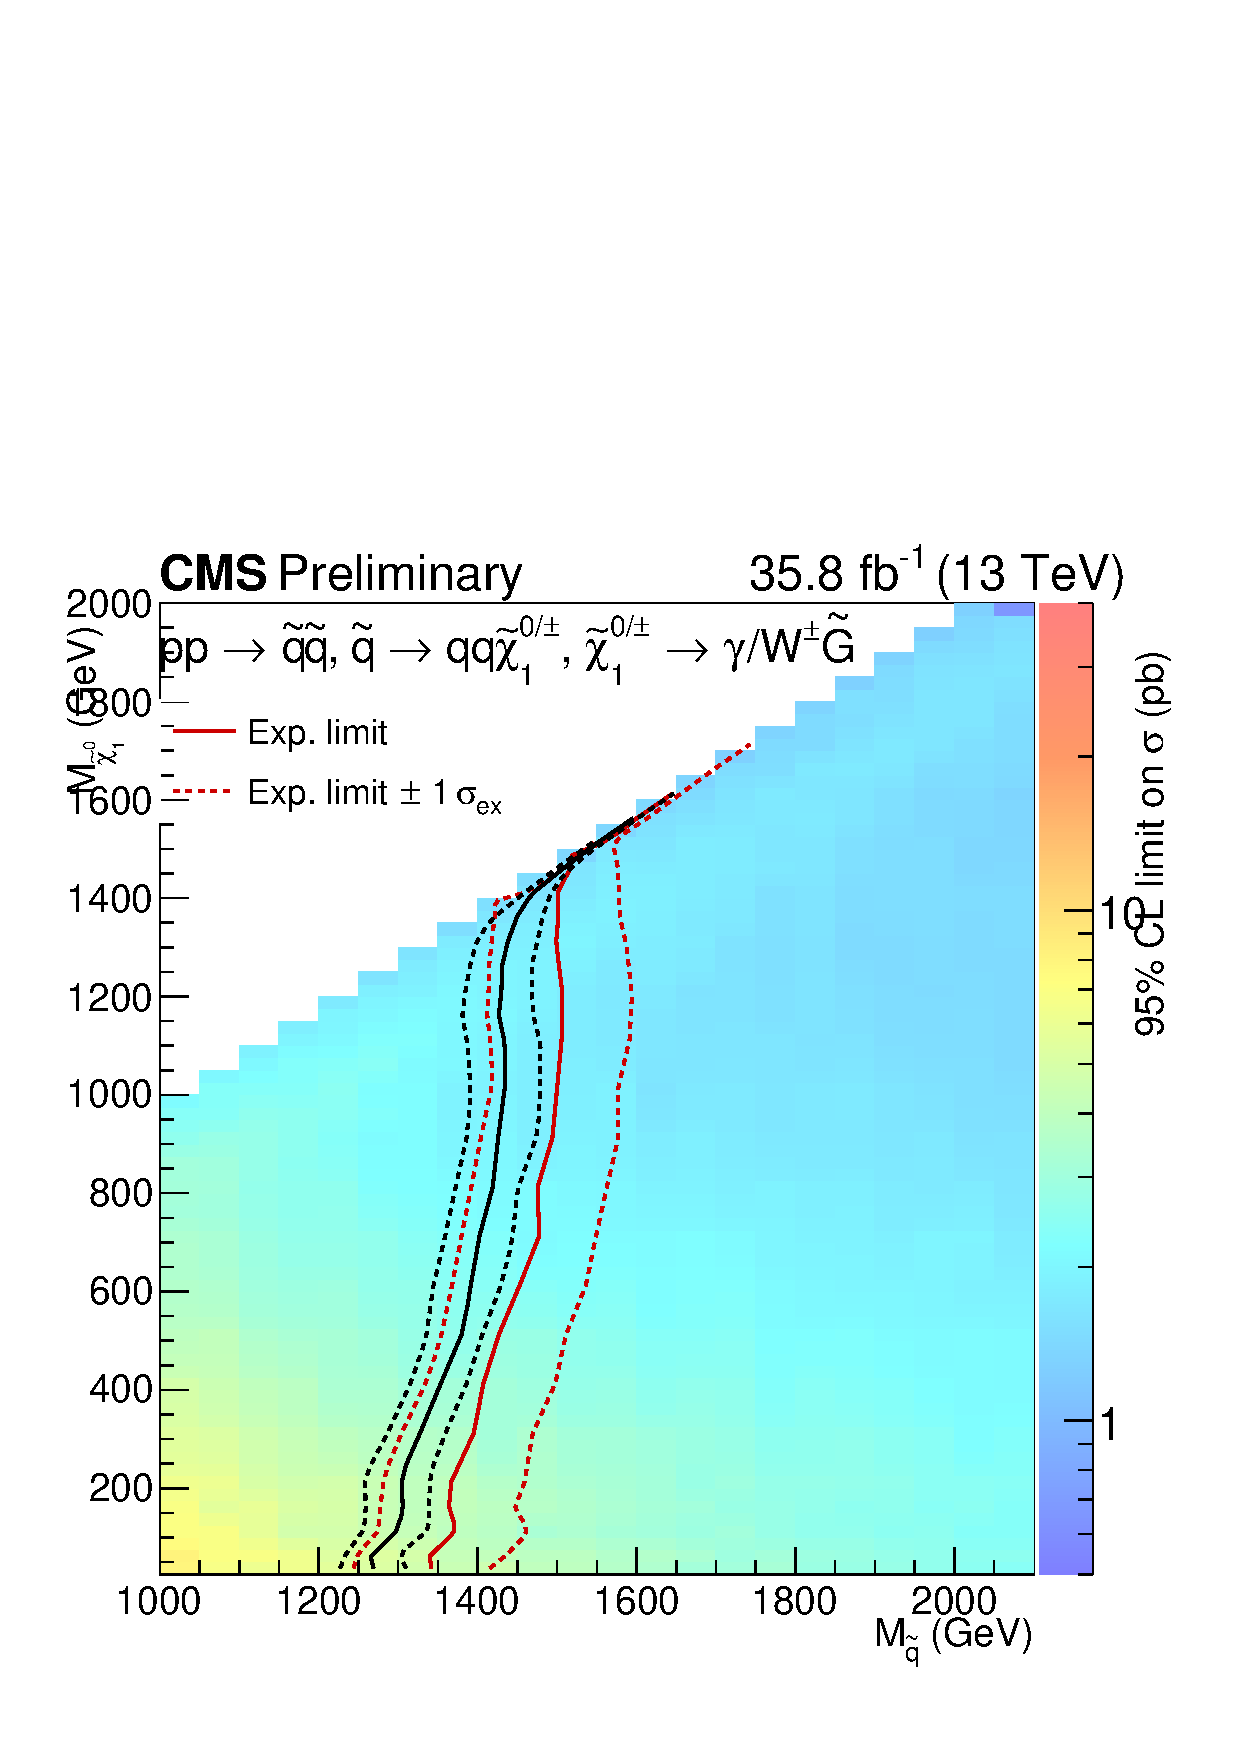
\includegraphics[width=0.49\textwidth]{Figures/T6WG_UnblindLimit_100_400_200.pdf} 
		\caption{Observed and expected exclusion limits for T5Wg (left) and T6Wg (right) models. The upper limits are set on the cross section $\times$ BR, where BR is the branching fractions to the neutralino/chargino states. For simplicity, BR is assumed to be 50\%. }
    \label{fig:t5wglimit}
\end{figure}

\end{document}
